\section{Introduction}

In modern web development environments, you need to have at least two types of tools:

\begin{itemize}

\item{\textbf{Compilers:} As most browser vendors have not yet implemented the new ES6 standard natively and many developers want to use one of the numerous compile-to-javascript languages that are rising in popularity, you need a compiler to transform the source code into the ES5 Javascript standard, which most browser are able to execute. The most popular compilers are \textit{Babel} for ES6, \textit{TSC} for Typescript and \textit{purs} for Purescript.}

\item{\textbf{Bundlers:} Because until ES6 Javascript did not have a syntax to import modules for other source files and browser vendors have not yet implemented this syntax, you need bundlers that link your code together, provide dependencies and bootstrap your application. Some also generate the \textit{index.html} file with all assets linked or included. The most popular bundler is \textit{webpack}. Other solutions are \textit{rollup} and \textit{browserify}}

\end{itemize}

The seperation between those two creates a few problems:

\begin{itemize}
\item{It is not possible to optimize across modules, because the compiler is not aware of the other modules' AST}

\item{The bundler has to introduce a runtime to wrap the compiled output, because it is not aware of the AST of the code}

\item{It is not easy to use multiple lanugages, especially running tests written in multiple languages is hard as testing tools expect Javacript input}

\item{New syntaxes have to be added to all languages individually, for example JSX which was introduced by Facebook and not usable in Typescript for a long time, because Facebook only implemented support in Babel}

\end{itemize}

The fact that most tools are written in Javascript also leads to problems, because Javascript only has limited concurrency and is slow to execute even with modern virtual machines (VM).

To fix those problems, the goal of this paper is to develop a new compiler whose design allows being extended by modules to add new syntaxes to existing languages with minmal efford. To make implementation easier and performance better, the compiler called \textit{pack.hs} will be written in Haskell.

\section{Design of the compiler}

\subsection{Dynamic AST definition}

The compiler should allow plugins to add syntax to the definitions of other plugins. This means that every plugin, be it a core plugin implementing a certain language like Typescript or an extention plugin that augments existing core plugins, is allowed to add grammar to the AST definition.

One example here would be a JSX plugin on top of a Javascript plugin. JSX is syntax made pobular by Facebook with its React framework. It allows for a HTML-like syntax as a normal Javascript expression, which is used by the framework to describe components to be rendered (see listing~\ref{lst:jsx} as example).

\begin{lstlisting}[caption={Simple JSX view function}, captionpos=b, label=lst:jsx]
function view(state) {
    return (
        <div>
            <span>{ state.myValue }</span>
        </div>
    );
}
\end{lstlisting}

The same syntax is also useful in Typescript, as Typescript is a typed superset of Javascript. So in an ideal case the JSX plugin should work without modifications with both source languages.

As the used plugins are configured at runtime, the final AST definition is not known at runtime. A core plugin should be able to be used together with a extention plugin that was written after the core plugin without having to modify or recompile the core plugin.

To allow this, the compiler only has one abstract data type (ADT) representing a grammar in  augmented Backus--Naur form (ABNF, see listing~\ref{lst:ABNF} as example). The plugins provide grammar files that are then parsed by the compiler to construct the final AST (see section~\ref{sec:pipeline}).

\begin{lstlisting}[linewidth=\columnwidth, caption={Simple example of ABNF grammar}, captionpos=b, label=lst:ABNF]
S ::= function;
function ::= 'function' IDENTIFIER '(' [arguments] ')' block;
arguments ::= argument [additionalArguments];
additionalArguments ::= ',' argument [additionalArguments];
argument ::= IDENTIFIER typeDeclaration | IDENTIFIER;
block ::= '{' statement* '}';
typeDeclaration ::= ':' type;
type ::= 'boolean' | 'string' | 'number';
statement ::= 'return' expression [';'];
literal ::= '"' LITERAL '"' | LITERAL | 'true' | 'false';
expression ::= literal | expression operator expression;
operator ::= '+' | '-' | '===';
\end{lstlisting}

This grammar represents a small subset of Typescript. A similar grammar is used in the current implementation.

\subsection{Compiler pipeline}
\label{sec:pipeline}

A classic compiler is implemented as a pipeline of three to five distinct parts (see figure~\ref{fig:compiler_pipeline}).

\begin{figure}[H]
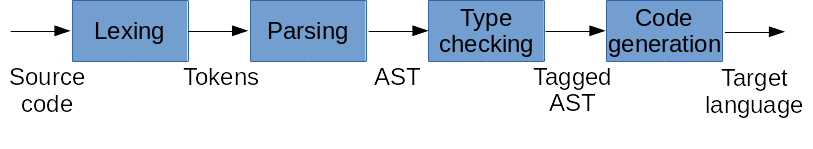
\includegraphics[width=\columnwidth]{./compiler_pipeline.png}
\caption{A classic compiler pipeline}%
\label{fig:compiler_pipeline}
\end{figure}

The lexing step takes the source code to be parsed, together with a Chomsky type 3 grammar that is used to split the raw input string into a ordered set of tokens. This step can be left out, if the characters in the input string are seen as tokens individually.

A Parser then takes those tokens and a Chomsky type 2 grammar to parse an AST\@. This AST can optionally be type checked before it is transformed into the target language. In the context of the web, this most likely Javascript.

In the code generation step, the AST is written into a target file, for Javascript this is another text file. Most of the time this also includes a minification step, where the compiler replaces names with short, obfuscated versions and omits as much whitespace as possible.

The compiler described in this paper also uses a pipeline approach, but with different steps (see figure~\ref{fig:pack.hs_pipeline}).

\begin{figure}[H]
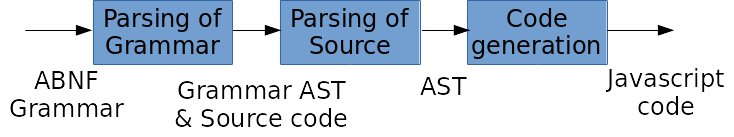
\includegraphics[width=\columnwidth]{./pack_hs_pipeline.png}
\caption{Compiler pipeline in pack.hs}%
\label{fig:pack.hs_pipeline}
\end{figure}

Here the compiler first collects the grammar files from the plugins. In the current proof of concept implementation, this is just one typescript syntax file. Those grammars are then parsed into a special ABNF grammar AST\@.

This AST is then used to generate a source code parser at runtime, which takes the source code and parses it into an AST\@. To simplify the implementation, there is no type checking done yet. This AST is piped through a bunch of transforming functions which come from the plugins. Those transforms are what compiles the code.

The last step again is code generation, which transforms the AST into obfuscated and minified Javascript code.

\section{Implementation}

\subsection{Host language}

The compiler is written in Haskell, because of several advantages:

\begin{itemize}

\item{The lazy nature of Haskell allows for easy parsing of self-recursive grammars}
\item{Later in the project, the compiler can make use of the parallelism built into the Haskell runtime to compile multiple files at the same time.}
\item{Haskell is a compiled language, so the final execution does not suffer performance hits introduced by parsing and interpreting}
\item{Haskell's strong type system makes debugging code a lot easier, because most of the errors are already caught by the compiler}
\item{GHCI, Haskell's interactive interpreting compiler allows to test functions in isolation before inserting them into the program}
\item{The monadic approach and the accompanying \textit{do} notation make composing complex parsers out of simple ones easy}
\item{Parsing libraries for Haskell are feature-rich and very mature, this compiler uses \textit{Megaparsec}}

\end{itemize}
